\chapter{Introduction}
 A PLL is a feedback system that includes a VCO, phase detector, and low pass filter within its loop.Its purpose is to force the VCO to replicate and track the frequency and phase at the input when in lock. The PLL is a control system allowing one oscillator to track with another ie. it keeps the an ouput signal synchronized with the reference signal in terms of frequency and phase.
\begin{equation}
    \label{eq:pll_1}
    \phi_{\text{out}}(t) = \phi_{\text{in}}(t) + \text{const.}
\end{equation}
\begin{figure}[h]
    % \vspace{-0.7cm}
      \centering
      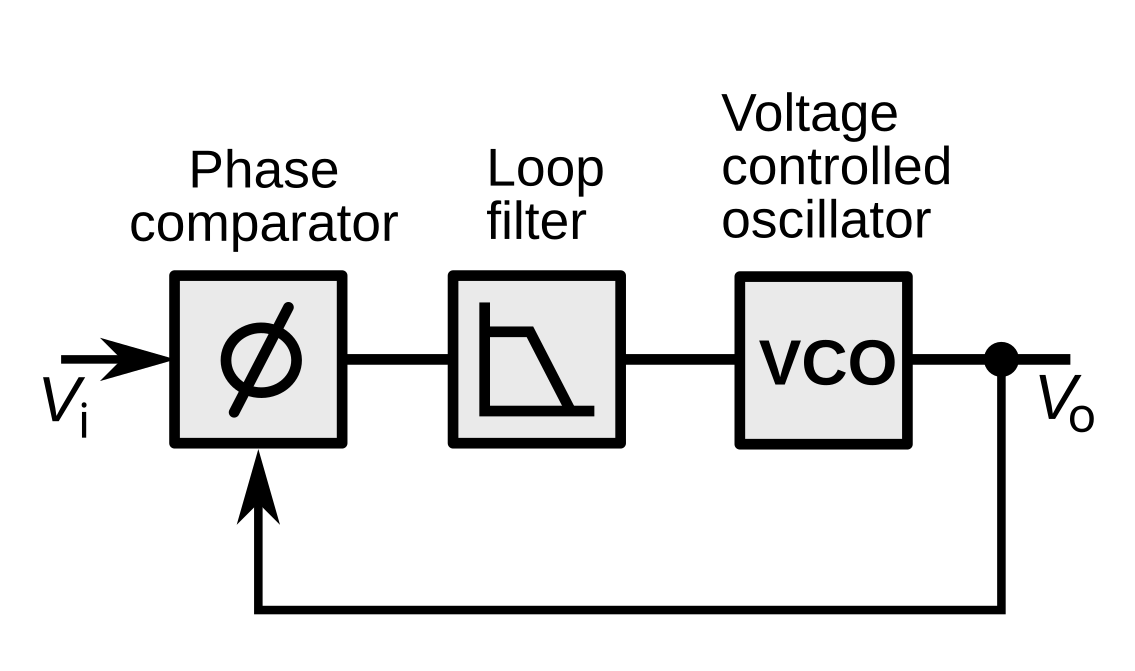
\includegraphics[width=0.5\textwidth]{figs/Phase_locked_loop.png}      \vspace{-0.3cm}
      \caption[]{ Simple analog phase locked loop}
      \label{fig:pll_1}
    % \vspace{0.5cm}
\end{figure}    
\section{Motivation}
Our team chose to work on the PLL project to gain practical knowledge about the fundamentals of phase-locked loops and their applications in modern electronics. We were particularly interested in the design and implementation of a PLL circuit at the transistor level to understand the underlying principles of PLL operation and the challenges involved in designing such circuits. We were motivated by the opportunity to work with simulation tools and techniques, such as LTspice, to analyze and optimize.

\section{Brief History and Applications of PLL}
\begin{itemize}
    \item The PLL was invented in 1932 by Harold Stephen Black, an engineer at Bell Labs.
    \item The original PLL was used in telephone systems to eliminate noise and improve the quality of voice signals.
    \item Since then, the PLL has been widely used in various applications, including:
    \begin{itemize}
        \item Clock generation: Ensuring that all components operate synchronously.
        \item Frequency synthesis: Generating a range of frequencies from a single reference frequency.
        \item Demodulation: Used in communication systems like FM radio and digital communication systems.
        \item Data recovery: Recovering clock signals from data streams for proper synchronization.
        \item Jitter reduction: Improving the performance of high-speed digital circuits.
        \item Phase alignment: Aligning the phase of multiple signals for proper timing and synchronization.
        \item Frequency modulation: Modulating signals in communication systems like FSK and PSK.
        \item Signal conditioning: Filtering and conditioning signals to improve quality and reduce noise.
        \item Clock recovery: Ensuring proper synchronization between transmitting and receiving devices.
    \end{itemize}
\end{itemize}

\section{Objective of the Project}
\begin{itemize}
    \item To design a PLL circuit at the transistor level using LTspice, with specific characteristics and specifications.
    \item Design targets:
    \begin{itemize}
        \item Reference Frequency = 20 MHz
        \item Output Frequency = 2.4 GHz
        \item Power Consumption = 2 mW
        \item Deterministic Jitter = 10 ps, pp
        \item Random Jitter = 2 ps, rms
        \item Supply Voltage = 1 V
    \end{itemize}
    \item Carry out simulations to verify the performance of the designed PLL circuit.
    \item Analyze the results and compare them with the design targets.
    \item Identify the charachteristics of the PLL circuit for example:
    \begin{itemize}
        \item Phase noise
        \item Jitter
        \item Lock time
        \item Frequency stability
        \item Power consumption
        \item Output waveform
        \item Phase margin
        \item Loop bandwidth
        \item frequecy capture range
    \end{itemize}       
    \item Document the design process, challenges faced, and lessons learned during the project.
\end{itemize}